\documentclass[10pt,a4paper]{article}
% Shared layout for the two reading guides (vademecum) that accompany the decks.
\usepackage[T1]{fontenc}
\usepackage[utf8]{inputenc}
\usepackage[english]{babel}
\usepackage{mathpazo}
\usepackage{amsmath,amssymb,bm,booktabs,array,graphicx,microtype,xcolor}
\usepackage[a4paper,left=14mm,right=14mm,top=11mm,bottom=14mm]{geometry}
\usepackage{titlesec,enumitem,siunitx}
\usepackage[most]{tcolorbox}
\tcbuselibrary{raster}
\usepackage[colorlinks=true,urlcolor=accent,linkcolor=accent]{hyperref}
\sisetup{group-separator={,},group-minimum-digits=4}
\definecolor{pisablue}{RGB}{74,96,121}
\definecolor{pisablight}{RGB}{192,206,220}
\definecolor{accent}{RGB}{26,118,179}
\definecolor{expert}{HTML}{C98A1E}
\definecolor{muted}{HTML}{666666}
\titleformat{\section}{\color{pisablue}\bfseries\normalsize}{\thesection}{.6em}{}
\titlespacing*{\section}{0pt}{1.6ex plus .4ex}{.5ex}
\titleformat{\subsection}[runin]{\color{pisablue}\bfseries\small}{}{0pt}{}[.]
\titlespacing*{\subsection}{0pt}{.7ex}{.5em}
\setlist{nosep,leftmargin=1.2em,topsep=.2ex}
\setlength{\parindent}{0pt}
\setlength{\parskip}{.45ex}
\pagestyle{plain}
\newtcolorbox{summarybox}{enhanced,colback=pisablight!22,colframe=pisablue!60,boxrule=.4pt,arc=0pt,left=5pt,right=5pt,top=3pt,bottom=3pt,fontupper=\small}
\newtcolorbox{paperbox}[1][]{enhanced,colback=pisablight!18,colframe=pisablue!55,boxrule=.4pt,arc=0pt,left=5pt,right=5pt,top=2pt,bottom=3pt,fontupper=\small,
 title={In the paper#1},fonttitle=\bfseries\small,coltitle=pisablue,colbacktitle=pisablight!18,titlerule=0pt,toptitle=2pt,bottomtitle=0pt}
\newtcolorbox{ideabox}{enhanced,colback=expert!8,colframe=expert,boxrule=.5pt,arc=0pt,left=5pt,right=5pt,top=2pt,bottom=3pt,fontupper=\small,
 title={Proposals, not in the paper},fonttitle=\bfseries\small,coltitle=expert!70!black,colbacktitle=expert!8,titlerule=0pt,toptitle=2pt,bottomtitle=0pt}
% \vademecumheader{title}{authors}{journal}{doi, URL-encoded}{doi as printed}{companion deck}
\newcommand{\vademecumheader}[6]{%
 {\color{pisablue}\large\bfseries #1\par}\vspace{.6ex}
 {\small #2\enspace\textperiodcentered\enspace #3\par}
 {\footnotesize\href{https://doi.org/#4}{doi:#5}\par}
 {\footnotesize\color{muted} Reading guide by Matteo Di Sante for the paper review; companion deck: #6. Equation, figure and section numbers are those of the paper.\par}\vspace{.8ex}}
\newcommand{\ours}{{\color{expert!70!black}\bfseries[ours]}}

\hypersetup{pdftitle={Reading guide: Neggers, Jonker and Siebesma (2003)},pdfauthor={Matteo Di Sante}}

\begin{document}
\vademecumheader{Size statistics of cumulus cloud populations in large-eddy simulations}
{R.\,A.\,J. Neggers, H.\,J.\,J. Jonker, A.\,P. Siebesma}
{J. Atmos. Sci. \textbf{60}, 1060--1074 (2003)}
{10.1175/1520-0469(2003)060\%3C1060:SSOCCP\%3E2.0.CO;2}
{10.1175/1520-0469(2003)060<1060:SSOCCP>2.0.CO;2}
{\texttt{neggers2003.pdf} (5 slides)}

\begin{summarybox}
\textbf{In brief.} Large-eddy simulations (LES) of three shallow-cumulus cases are analysed with the method of satellite studies. The cloud size density is a power law, $\mathcal N(l)\propto l^{-1.70}$, from the grid spacing up to a scale break $\ell_d$ (400--\num{1250} m), above which it falls steeply. Rescaled by $\ell_d$, all cases collapse: $\ell_d$ is the only case-dependent parameter. Since the exponent is above $-2$ below the break and below $-2$ above it, the projected cloud cover and the vertical mass flux are dominated by clouds of intermediate size, near $\ell_d$, not by the numerous small clouds, which carry almost no mass flux. These results hold for grids of 25--100 m; too small a domain truncates the spectrum, and shear moves $\ell_d$ while leaving the total mass flux unchanged. What sets $\ell_d$ is left open.
\end{summarybox}

\section{Context and motivation}
General circulation models must parameterize broken shallow-cumulus fields twice. Radiation schemes need the geometry of the field, and mass-flux convection schemes (Arakawa \& Schubert 1974; Tiedtke 1989) need the vertical transport of heat, moisture and momentum, written through entrainment and detrainment rates that theories relate to cloud size. Observations disagree on the form of the \emph{cloud size density}, the pdf of the number of clouds as a function of size: exponential (Plank 1969; Wielicki \& Welch 1986), lognormal (L\'opez 1977) or power law (Cahalan \& Joseph 1989; Kuo et al.\ 1993; Benner \& Curry 1998). The last three report a scale break, which Cahalan \& Joseph relate to the largest convective cells of the boundary layer. Observed cloud fraction is dominated by an intermediate, well-defined size: small clouds are many but cover little, large ones are rare. Aircraft and radar measure vertical velocity, needed for the mass flux, in only a few clouds.

LES offers full 3D, time-dependent fields, statistics limited only by computing time, and complete control of the case. It reproduces bulk transport well in GCSS intercomparisons; whether it resolves the individual clouds that matter was unknown. Earlier LES size distributions were limited by resolution (Beniston \& Sommeria 1981) or found to depend on it (Brown 1999b).

\section{Aims}
(1) Compare LES size densities with observed ones, using the same algorithm and a comparable number of clouds. (2) Test whether one functional form with few parameters fits all cases, by looking for typical scales. (3) Use the link between the density and the size decompositions of cloud fraction and mass flux to find which sizes contribute most. (4) Test sensitivity to resolution, domain size and vertical wind shear.

\section{Model and cases}
KNMI LES (Cuijpers \& Duynkerke 1993): filtered equations in the inertial subrange, centred advection, a prognostic equation for subgrid turbulent kinetic energy, subgrid length $\ell_0\sim(\Delta x\Delta y\Delta z)^{1/3}$. A 3D field is sampled every 5 min; several runs with randomized initial temperature give independent statistics.

\smallskip
{\small\setlength{\tabcolsep}{4pt}\begin{tabular}{@{}lp{76mm}ccccr@{}}
\toprule
Case & Setting & $\Delta x$, $\Delta z$ (m) & Domain (km) & $Q_H$, $Q_L$ (W\,m$^{-2}$) & Clouds\\
\midrule
BOMEX & Trade-wind cumulus over ocean, steady state; subsidence balances the clouds; 10 runs, first 3 h discarded & 50, 40 & $6.4^2\times3$ & 8, 150 & \num{36776}\\
SCMS & Florida, 5 Aug 1995, over land; $\sim$1.5 km cloud layer, deepening; wind $(-4,4)$ m\,s$^{-1}$ & 50, 40 & $6.4^2\times5$ & 150, 300 & \num{20268}\\
ARM & Oklahoma (SGP), 21 Jun 1997, over land; full diurnal cycle; clouds from 1430 UTC, fluxes peak at 1900 UTC & 66.7, 40 & $6.4^2\times4.4$ & 140, 500 (max) & \num{35137}\\
\bottomrule
\end{tabular}}
\smallskip

\section{Definitions (Section 3 and Appendix)}
A grid box is cloudy if saturated; an offline algorithm splits each 3D field into $N$ connected clouds. The vertically projected field of cloud $n$ is $c_n^p(i,j)=H\big[\sum_kc_n(i,j,k)\big]$, its projected area $A_n^p$, and its size
\[
 \ell_n=\sqrt{A_n^p},\qquad N=\int_0^\infty\!\mathcal N(l)\,dl,\qquad a^p=\int_0^\infty\!\alpha^p(l)\,dl,\quad \alpha^p(l)=\frac{l^2\,\mathcal N(l)}{L_xL_y},
\]
the same definition as in satellite images. With the cloud fraction $\alpha(l,z)$ and cloud-mean velocity $w(l,z)$ of size class $l$ at height $z$, the mass flux is $m(z)=a(z)\,w(z)$, $\mu(l,z)=\alpha(l,z)\,w(l,z)$, and its cloud-layer average is $\mu(l)=h_c^{-1}\int_{h_c}\mu(l,z)\,dz$, $m=\int\mu\,dl$ (Eqs.\ 5--7). Each cloud keeps its projected size at every height, so it stays in one bin. The fit is $\mathcal N=a\,l^b$ (Eq.\ 8); a scale break is where $b$ changes. Histograms use linear bins but are plotted as $\mathcal N^*(\log l)=l\ln10\,\mathcal N(l)$ (Eq.\ 9), whose log--log slope is $b+1$. Projected cover differs from cover at one level because clouds overlap.

\section{Results}
\subsection{Size density (Figs.\ 4--6, Table 2)} The normalized densities of the three cases collapse at small sizes, with a constant slope over more than a decade, from the grid spacing to a distinct break. Lognormal and exponential forms would curve on log--log axes, so a power law is fitted: $\mathcal N^*/N=1.121-0.70\log l$, i.e.\ $b=-1.70$, robust through the ARM day. Observed values: log-bin slope $-0.89$ for remotely sensed clouds (Cahalan \& Joseph 1989); mean $b=-1.98$ with spread for tropical shallow cumulus (Benner \& Curry 1998). Break sizes: BOMEX 700 m, SCMS \num{1050} m, ARM 400, 700, \num{1000}, \num{1100}, \num{1250} m in successive hours from 15--16 to 19--20 UTC. A convergence test with more clouds moves neither the break nor the histogram above it. Dividing sizes by $\ell_d$ collapses all cases over all sizes (Fig.\ 6): a universal form with $\ell_d$ as the only variable, with another exponent or form above the break. Candidate controls of $\ell_d$: the depth of the (sub)cloud layer (suggested by ARM), the largest boundary-layer cells (Cahalan \& Joseph), and subcloud humidity fluctuations, whose filtering changed the typical cloud size dramatically in Jonker et al.\ (1999).

\subsection{Dominant size (Figs.\ 5, 7, 8; Table 3)} $\alpha^p/N$ collapses too, and peaks at the break. For a pure power law, Eq.\ (10) gives $\alpha^p(l)\propto l^{\,b+2}$: the smallest clouds dominate if $b<-2$, the largest if $b>-2$. With $b=-1.70$ below and $b<-2$ above $\ell_d$, the dominant size is intermediate and equals the break, as in observed fields. One-grid-box clouds cover somewhat too much area, probably a numerical effect. The mass-flux decomposition $\mu(l)$ peaks at larger sizes and more sharply, because the cloud-mean $w$ grows with size; the smallest clouds carry almost no mass flux. Totals: $a^p=14.15$, 26.72, 23.27\% and $m=0.015$, 0.060, 0.043 m\,s$^{-1}$ (BOMEX, SCMS, ARM 19--20 UTC). With height (Fig.\ 8): at cloud base ($z=600$ m) clouds below 200 m dominate the cover; higher up large clouds take over, since small clouds do not rise far; the largest clouds keep a roughly constant fraction and their mass flux grows slightly with height.

\subsection{Resolution (Fig.\ 9, Table 4)} BOMEX with $\Delta x=25$, 50, 100 m: the smallest clouds are always the most numerous and the scaling seems to continue below the grid scale (another decade would need 1--2 m grids). The cover of the smallest clouds tends to zero at finer grids, while the position and amplitude of the dominant size, and the largest size, do not change, even at 100 m. $a^p=14.48$, 14.15, 16.41\%; $m=0.0127$, 0.0145, 0.0162 m\,s$^{-1}$ for 100, 50, 25 m; the mass-flux increase comes from dominant and larger clouds and is attributed to poorer statistics of the largest clouds.

\subsection{Domain and shear (Figs.\ 10--11, Table 4)} In SCMS, the 3.2 km domain lacks the largest clouds of the 12.8 km run by the third hour, and dominance moves to the largest size. Shear ($\times0$, 1, 2) tilts clouds, enlarges projected sizes and broadens the density: $a^p=13.04$, 14.15, 19.38\% and $\ell_d$ grows, roughly as the maximum size; the total mass flux stays at 0.0145--0.0149 m\,s$^{-1}$, since the clouds still remove the conditional instability.

\subsection{Comparison with Brown (1999b) (Fig.\ 12)} Brown's decompositions moved to smaller sizes at finer resolution; these do not, even with his one-level, cross-section method at $z=900$ m. Suspected causes: sampling of the largest clouds, and the subgrid model (prognostic TKE here, Smagorinsky there).

\section{Authors' conclusions}
LES cumulus populations match natural ones; there is no evidence for exponential or lognormal densities. The power law is a robust geometric fingerprint whose physical explanation is open. The dominant clouds are far above the grid scale, hence resolved rather than subgrid. With $\ell_d$ as the only variable, parameterization is eased; what controls $\ell_d$ is unanswered.

\section{Limits}
\textbf{Stated or implied by the authors:} about one decade of scaling; unexplained break; domain-limited largest clouds; three shallow-cumulus cases only; comparison with nature through published exponents and dominant sizes, not the same scenes; the disagreement with Brown (1999b) unresolved. \textbf{Our reading} \ours: snapshot statistics, no cloud tracking or life cycle; no uncertainty on $b$, fitted by least squares on binned histograms; a cloud is saturated air, so rising air that never condenses is invisible.

\begin{tcbraster}[raster columns=2,raster equal height=rows,raster column skip=3mm,raster force size=false]
\begin{paperbox}[, on the subcloud layer]
Most large clouds root in the subcloud layer, which links $\ell_d$ to the cloud--subcloud interaction. Speculatively, two regimes: above the break, coherent structures of subcloud turbulence; below it, the decay of large clouds into smaller ones. In ARM, $\ell_d$ grows from 400 to \num{1250} m while the (sub)cloud layer deepens (Fig.\ 2).
\end{paperbox}
\begin{ideabox}
(1) Apply the same pipeline to climb crossings on a horizontal plane: connected patches, $\ell=\sqrt{\text{area}}$, $\mathcal N(\ell)$ in log bins; test for a power law, a break, and a collapse with boundary-layer depth. (2) Test whether the patch scale grows through the day, as $\ell_d$ does in ARM. (3) Build the analogue of $\mu(\ell)$ by weighting patches with climb rate times area. Caveat: pilots seek strong thermals and cross each one sparsely, so the sample is biased and incomplete.
\end{ideabox}
\end{tcbraster}

\par\vspace{1.2ex}\noindent
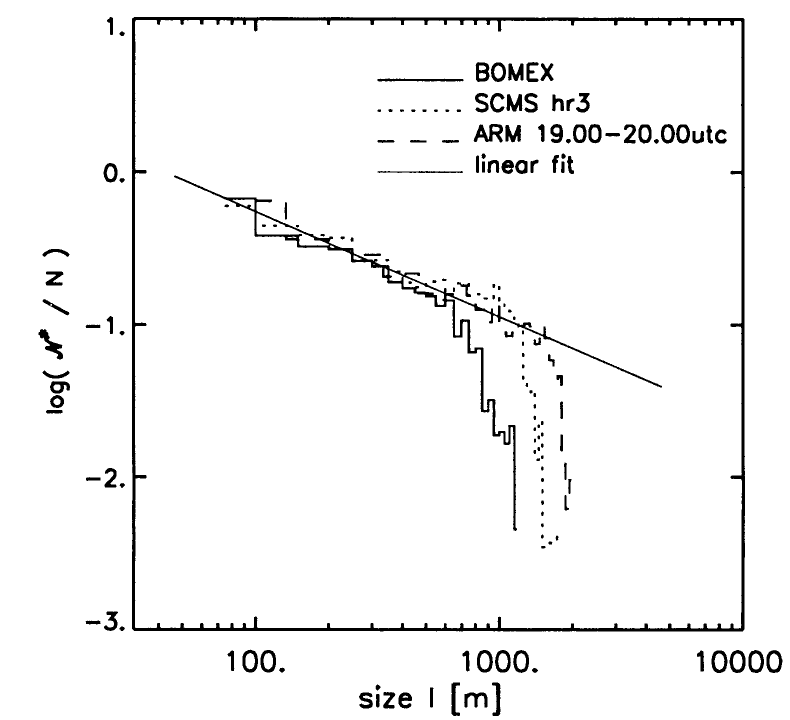
\includegraphics[height=28mm]{assets/neggers2003/fig4a.png}\hfill

\includegraphics[height=28mm]{assets/neggers2003/fig6.png}\hfill
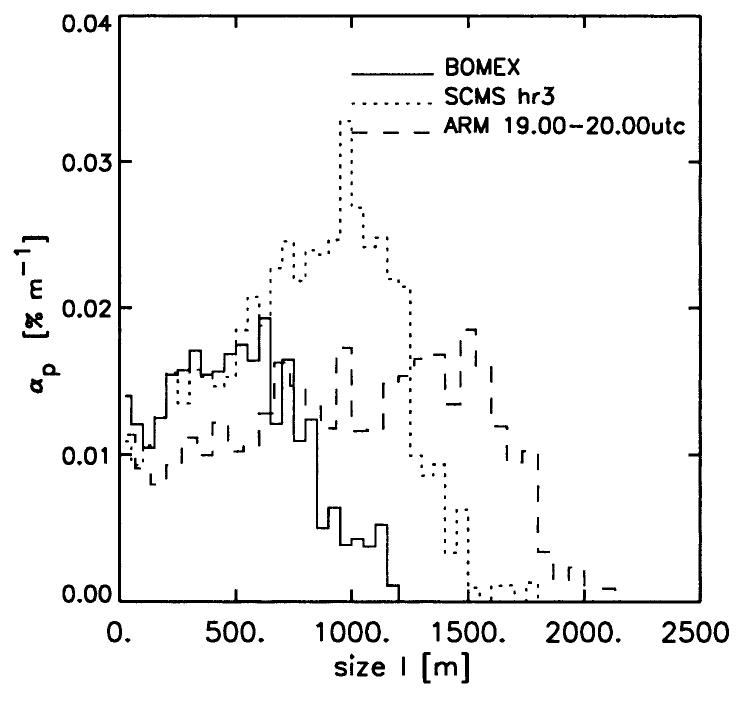
\includegraphics[height=28mm]{assets/neggers2003/fig7a.png}\hfill
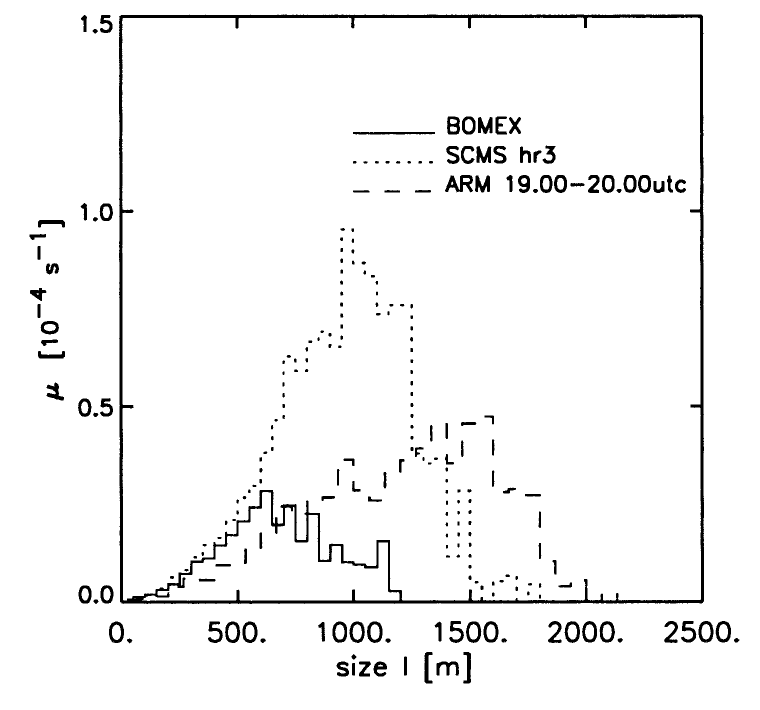
\includegraphics[height=28mm]{assets/neggers2003/fig7c.png}\par\vspace{.3ex}
{\footnotesize\color{muted}Key figures, reproduced from the paper. From left: Figs.\ 4a ($\mathcal N^*/N$ and fit), 6 (against $l/\ell_d$), 7a ($\alpha^p$) and 7c ($\mu$).\par}
\end{document}
